\documentclass{bioinfo}
\bibliographystyle{natbib}
%\bibliographystyle{achemnat}
%\bibliographystyle{plainnat}
%\bibliographystyle{abbrv}
%\bibliographystyle{bioinformatics}

\copyrightyear{2011}
\pubyear{2011}

\begin{document}
\firstpage{1}

\title[Knime4Bio]{Knime4Bio: a set of custom nodes for the interpretation of Next Generation Sequencing data with KNIME.}
\author[Pierre Lindenbaum \textit{et~al}]{Pierre Lindenbaum\,$^{1}$, Solena Le Scouarnec\,$^{2}$,  Vincent Portero\,$^{1}$ and Richard Redon\,$^{1,}$\footnote{to whom correspondence should be addressed}}
\address{$^{1}$Institut du thorax, Inserm UMR 915, Centre Hospitalier Universitaire de Nantes, 44000 Nantes, France.\\
$^{2}$The Wellcome Trust Sanger Institute, Hinxton, Cambridge CB10 1SA, UK.}

\history{Received on XXXXX; revised on XXXXX; accepted on XXXXX}

\editor{Associate Editor: XXXXXXX}

\maketitle

\begin{abstract}

\section{Summary:}
Analysing large amounts of data generated by next-generation sequencing (NGS) technologies is difficult for researchers or clinicians without computational skills. They are often compelled to delegate this task to computer biologists working with command line utilities. The availability of easy-to-use tools will become essential with the generalisation of NGS in research and diagnosis. It will enable investigators to handle much more of the analysis. Here, we describe Knime4Bio, a set of custom nodes for the KNIME (The Konstanz Information Miner) graphical workbench, for analysing some large NGS datasets using an interactive environment. We demonstrate that this tool can be utilised to quickly retrieve previously published scientific findings.

\section{Availability:}
\href{http://code.google.com/p/knime4bio/}{http://code.google.com/p/knime4bio/}.

\section{Contact:} \href{mailto:richard.redon@univ-nantes.fr}{richard.redon@univ-nantes.fr}
\end{abstract}

\section{Introduction}

Next-generation sequencing (NGS) technologies have led to an explosion of the amount of data to be analysed, for example a variant call format files (VCF~\citep{pmid21653522}, a standard specification for storing genomic variations in a text file)  produced by the 1000 genomes project contains about 25 million SNVs, making it difficult to extract relevant information using spreadsheet programs. Whilst computer biologists are used to invoke common command line tools - such as Perl and R - to analyse those data through Unix pipelines, scientific investigators generally lack the technical skills necessary to handle these tools and need to delegate data manipulation to a third-party. 
We have developed Knime4Bio, a set of new nodes  for the KNIME workbench~\citep{knimeref}. This modular environment enables an easy visual assembly and an interactive execution of an analysis pipeline. Nodes are mostly dedicated to the filtering and manipulation of VCF files. Although many standard nodes provided by KNIME can be used to perform such analysis, our nodes add new functionalities, some of which are described below. The nodes are written in Java, extend the classes of the KNIME API, are deployed and documented using a XML descriptor.

\section{Implementation}

To start with, VCF files are loaded in the working environment by providing an input file containing sample names and file paths.

Some nodes have been designed to find the intersection between the variants in the VCF file and a source of annotated genomic regions, which can be: a local BED file, a remote URL, a mysql table, a file indexed with tabix~\citep{pmid21208982}, a BigBed or a BigWig file~\citep{pmid20639541}.


Sets of key/value pairs can be extracted from the INFO or SAMPLE columns of the VCF file. For example, the sequence coverage or "depth", defined by a DP key in the INFO column, can be extracted and rows subsequently filtered with a standard numerical filter node according to the DP value: variants having a low or a high sequencing depth (hence having a higher probability of being false positives) can be removed.


Other new custom nodes allow the structure of a VCF table to be rearranged, by grouping the variants per sample or per gene. For example, a pivot table can be created, where each sample is assigned to a new column whilst each row represents a gene with an indication of the number of gene variants for each sample. The table also contains two additional summary columns, displaying the number of samples having at least one variant in each gene, and the number of distinct variants found in each gene. It is then possible to detect the genes harboring variants in a given number of samples.

Another node predicts the consequence of variations at the transcript/protein level. For each variant, genomic sequences of overlapping transcripts are retrieved from the UCSC knownGene database~\citep{pmid16500937} to identify variants leading to premature stop codons, non-synymous variants, and variants likely to affect splicing.

The Picard API~\citep{pmid19505943} is used to retrieve the aligned short reads overlapping a variant position from BAM files, that can be loaded in addition to the VCF files. A node then graphically displays short reads at the variation site, allowing the user to visually appreciate the quality of the variation.

Other nodes are able to incorporate data from other databases: dbSNFRP~\citep{pmid21520341}, dbSNP, Entrez Gene, PubMed, MediaWiki, the EMBL STRING database~\citep{pmid17098935}, Uniprot~\citep{pmid21447597}, Reactome~\citep{pmid21067998}, and GeneOntology~\citep{pmid18957448}, or to export the data to SIFT~\citep{pmid11337480}, Polyphen2~\citep{pmid20354512}, BED, or MediaWiki formats.

As a proof of concept we tested our nodes to analyse the exomes of six patients from a previously published study~\citep{pmid21378989} related to the Hajdu Cheney syndrome. For this purpose, short reads were mapped to the human genome reference sequence using BWA~\citep{pmid20080505} and variants were called using SAMtools mpileup~\citep{pmid19505943}. Homozygous variants, known SNPs (from dbSNP), and poor-quality variants were discarded, and only non-synonymous and variants introducing premature stop codons were considered. , On a redHat server(64bits, multicore, 4 processors , 2GB of RAM) our KNIME pipeline generated a list of 6 genes in 45 minutes: \href{http://www.ncbi.nlm.nih.gov/gene/9620}{\textit{CELSR1}},  \href{http://www.ncbi.nlm.nih.gov/gene/1284}{\textit{COL4A2}}, \href{http://www.ncbi.nlm.nih.gov/gene/64110}{\textit{MAGEF1}}, \href{http://www.ncbi.nlm.nih.gov/gene/51168}{\textit{MYO15A}}, \href{http://www.ncbi.nlm.nih.gov/gene/84905}{\textit{ZNF341}} and more importantly \href{http://www.ncbi.nlm.nih.gov/gene/4853}{\textit{NOTCH2}} the expected candidate gene (Fig.~\ref{fig:x1}).

\begin{figure}[!tpb]%figure1
\centerline{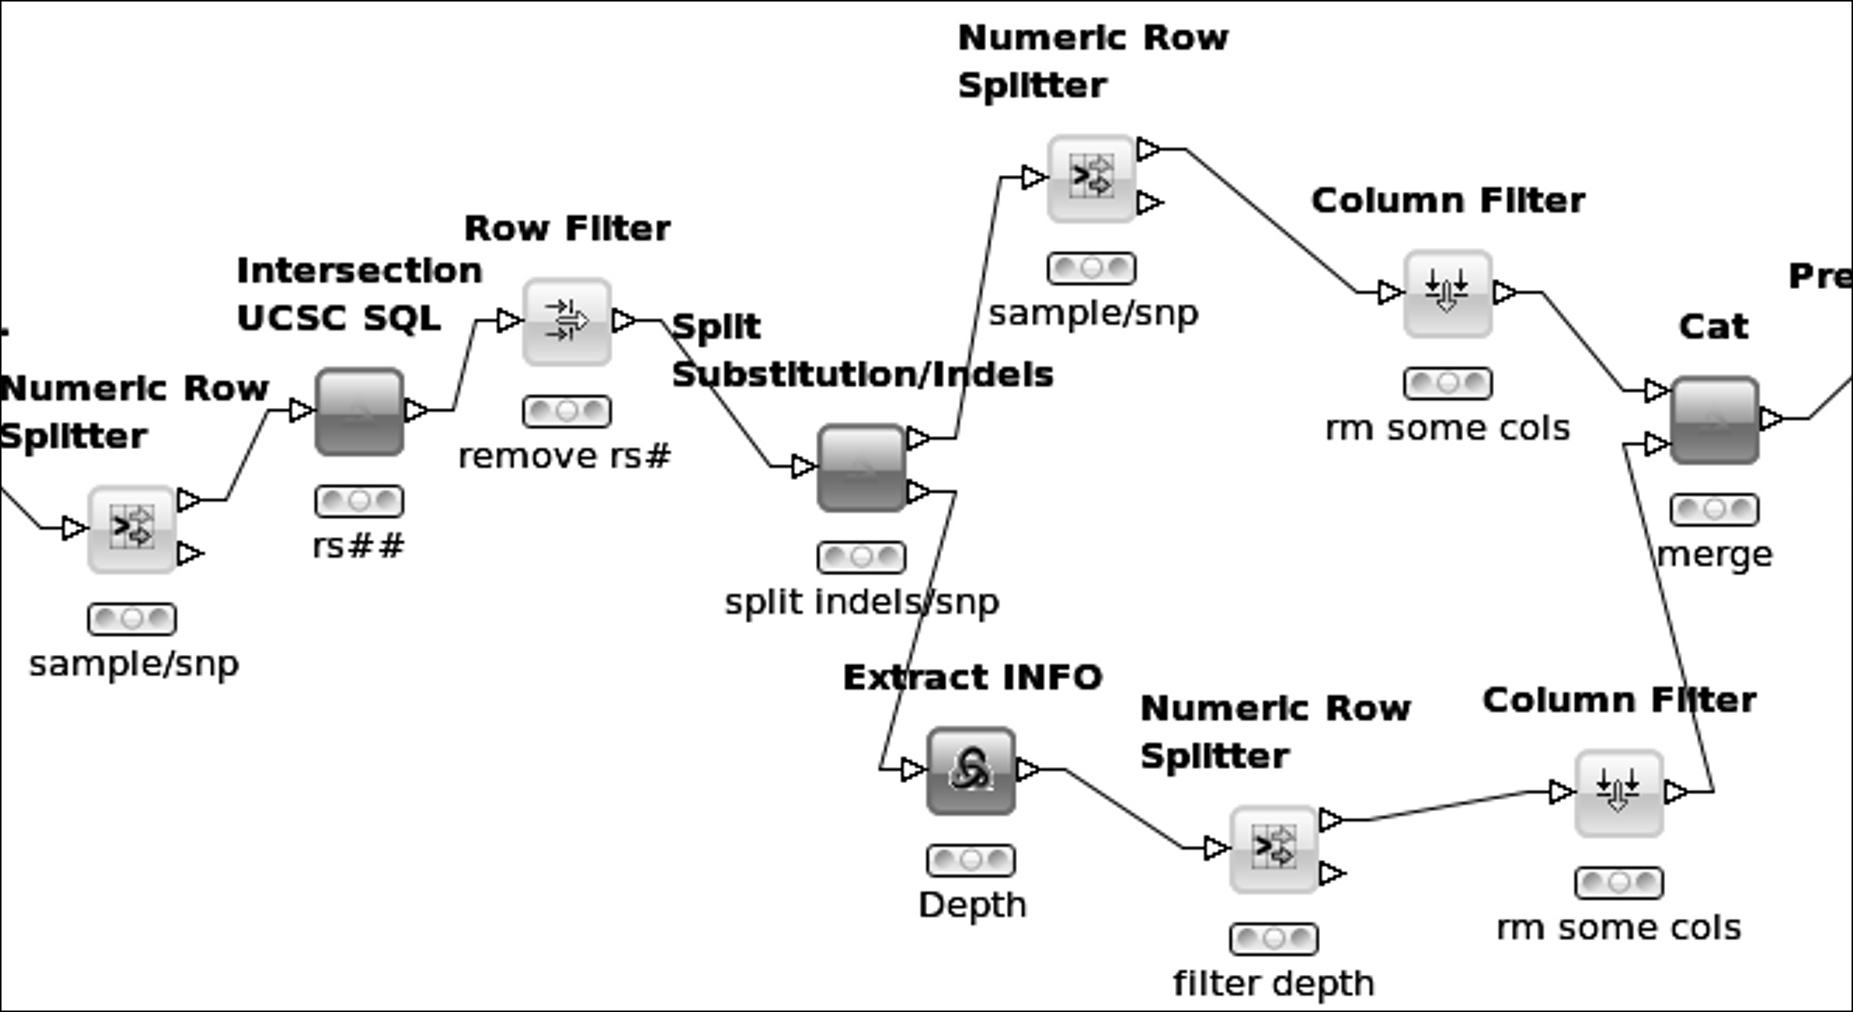
\includegraphics{fig01.eps}}
\caption{Screenshot of a Knime4Bio workflow.}\label{fig:x1}
\end{figure}

\section{Discussion}

Other workflow engines have been published such as Galaxy \citep{pmid21531983}, Mobyle~\citep{pmid19689959}, Taverna~\citep{pmid16845108} or Cyrille2~\citep{pmid18269742}. We found that KNIME is a lightweight solution and its programming interface seemed easier to implement. After a short tutorial and the construction of a basic workflow, the users were able to quickly play with the interface and modify the parameters without any further assistance. KNIME provides the ability to explore an idea by quickly dragging and modifying nodes without having to re-run the whole analysis. At the time of writing, Knime4Bio contains 54 new nodes. We believe Knime4Bio is an efficient and interactive tool for next-generation sequencing analysis.


\section*{Acknowledgements}
We want to thank the  \href{http://biostar.stackexchange.com/}{Biostar community} for its help, Jim Robinson and his team for the \href{http://code.google.com/p/bigwig/}{BigWig java API}, and Dr Cedric Le Caignec for the \textit{NOTCH2} data.

\paragraph{Funding\textcolon} This work was supported by the Inserm, the "Centre Hospitalier Universitaire" of Nantes, the "F\'{e}d\'{e}ration Fran\c{c}aise de Cardiologie" (FFC) and the "Fondation pour la Recherche M\'{e}dicale" (FRM).
\\


\bibliography{knime}

\end{document}
